% Editable native annotations around unchanged verified IDE photographs.
\par
\begin{figure}[htbp]
\centering
\sbox0{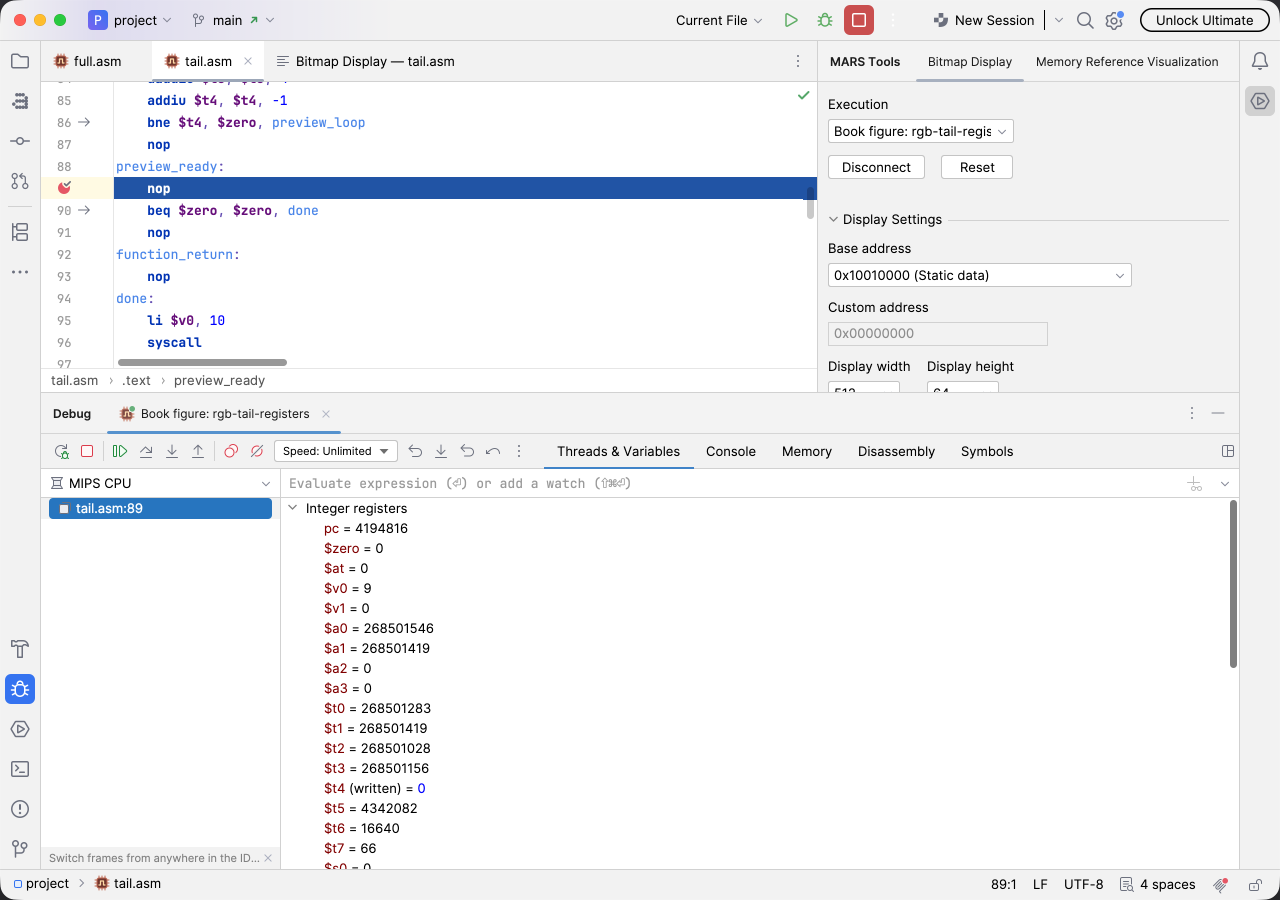
\includegraphics[artifact]{packages/019-rgb-formats/captures/f04/registers.png}}
\sbox2{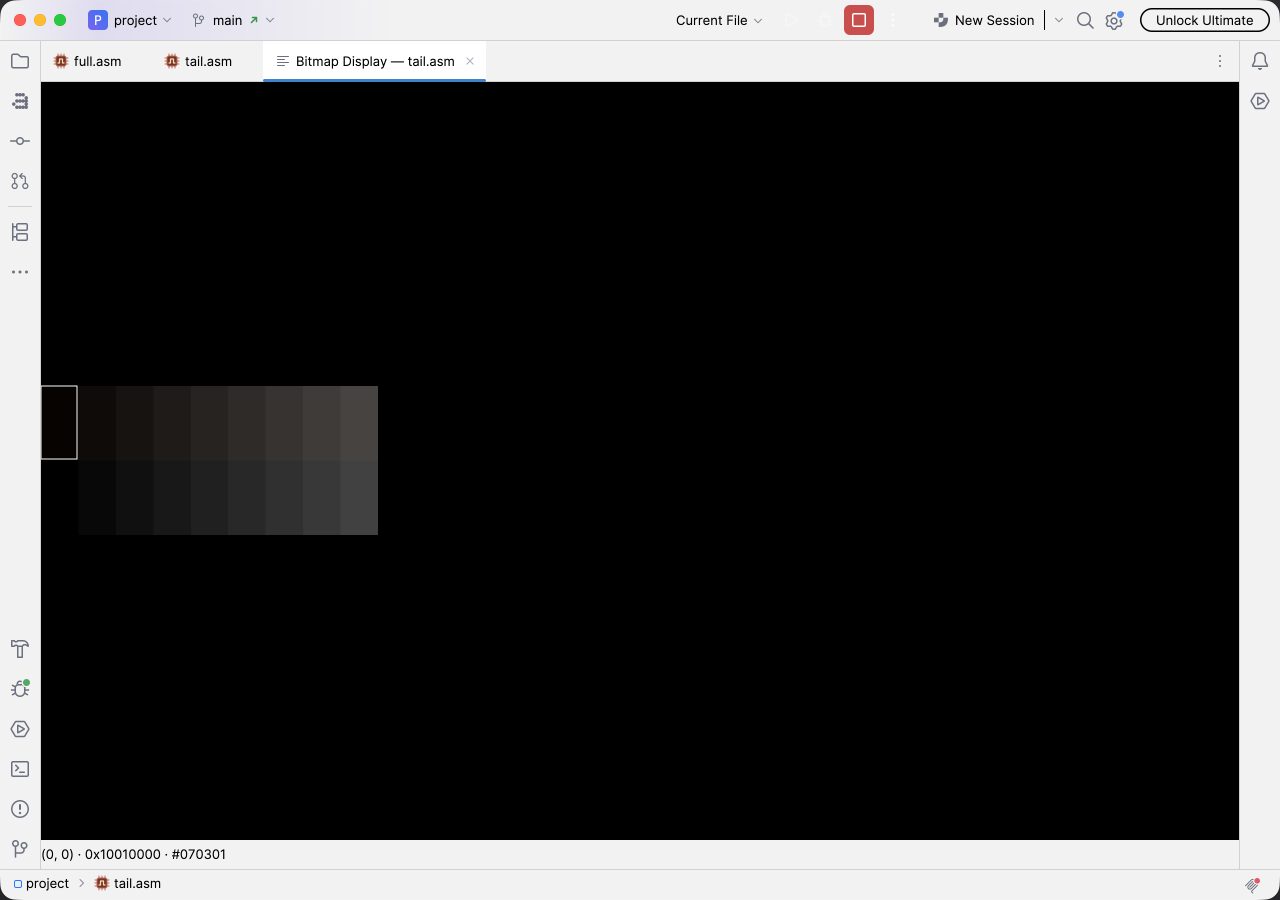
\includegraphics[artifact]{packages/019-rgb-formats/captures/f04/bitmap.png}}
\sbox4{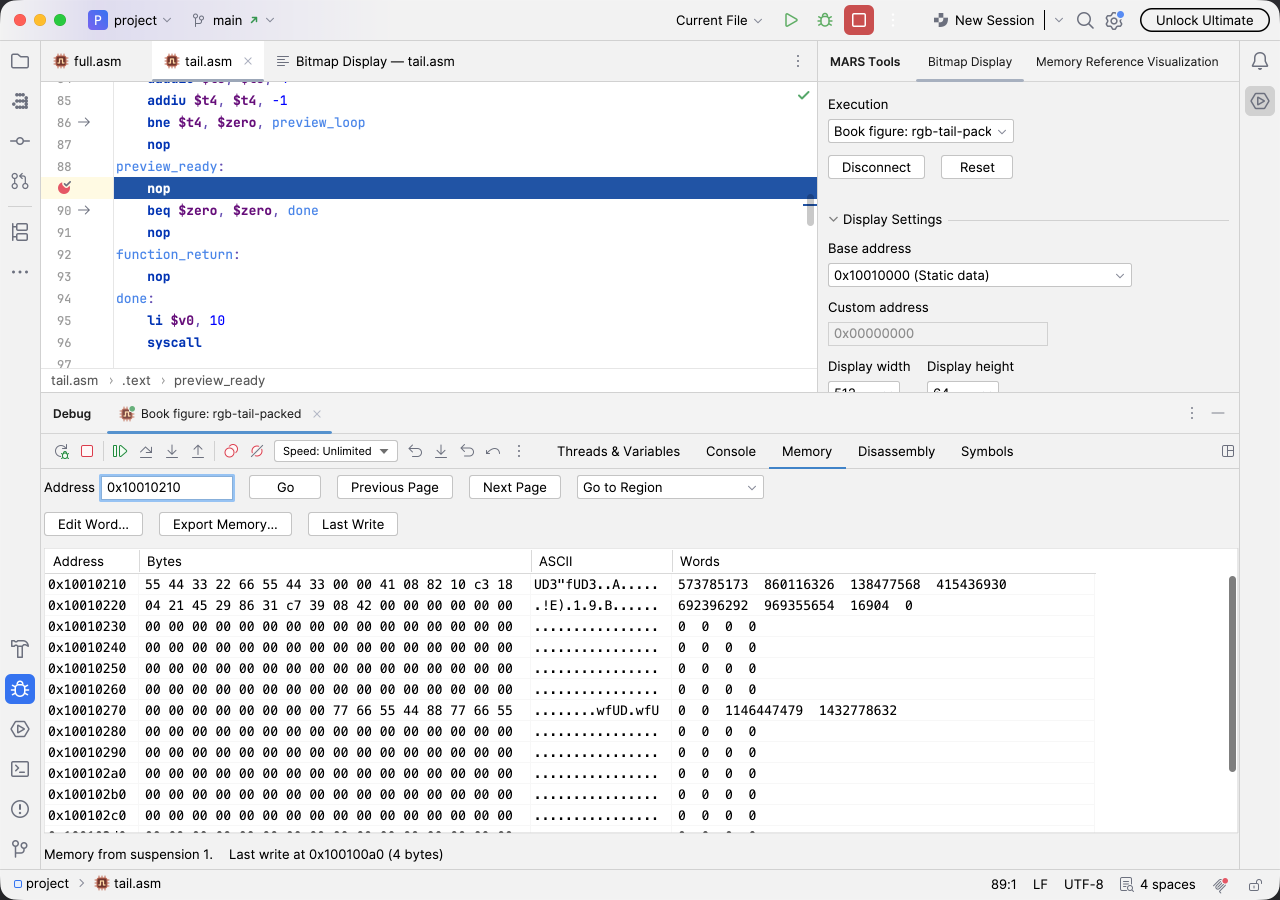
\includegraphics[artifact]{packages/019-rgb-formats/captures/f04/packed.png}}
\sbox6{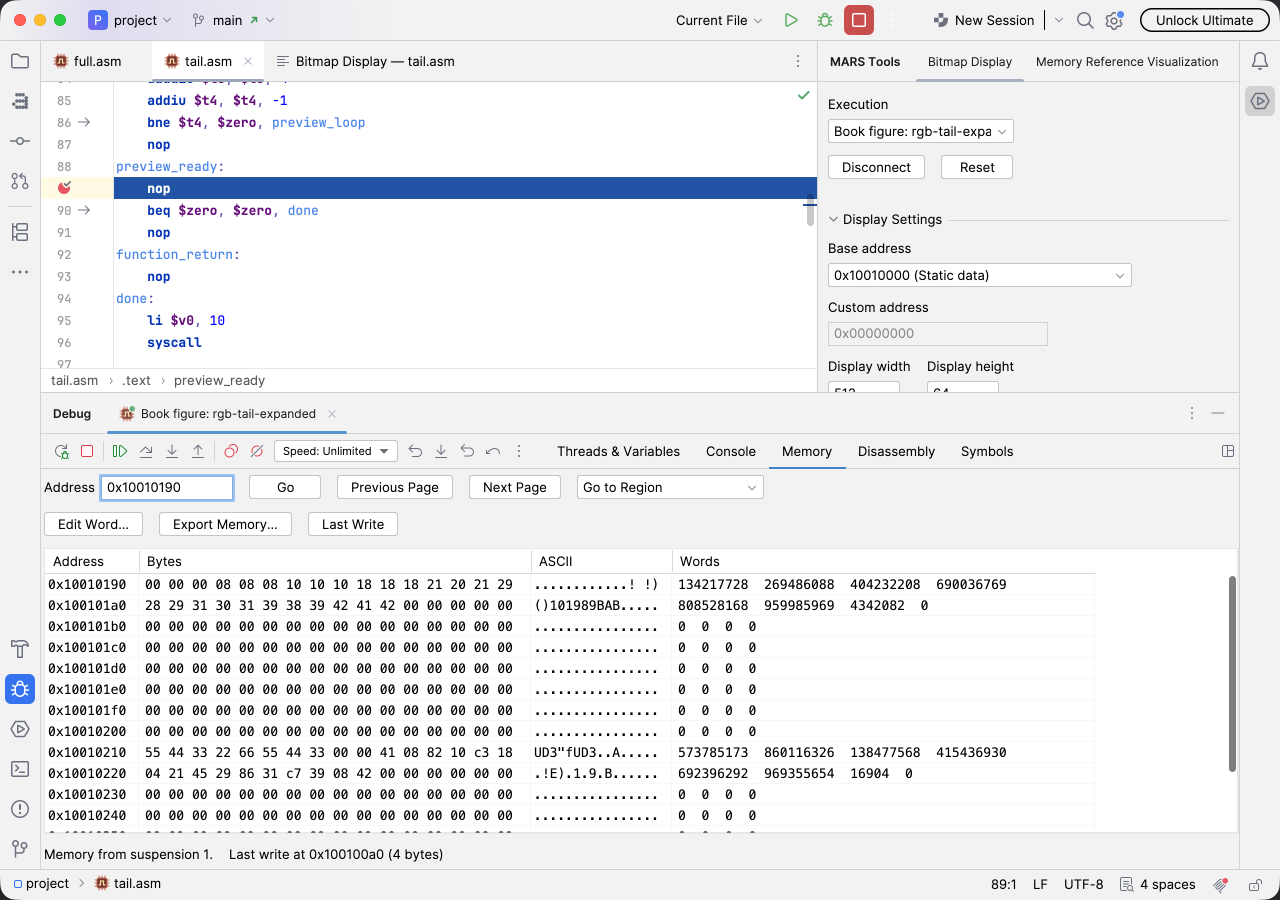
\includegraphics[artifact]{packages/019-rgb-formats/captures/f04/expanded.png}}
\sbox8{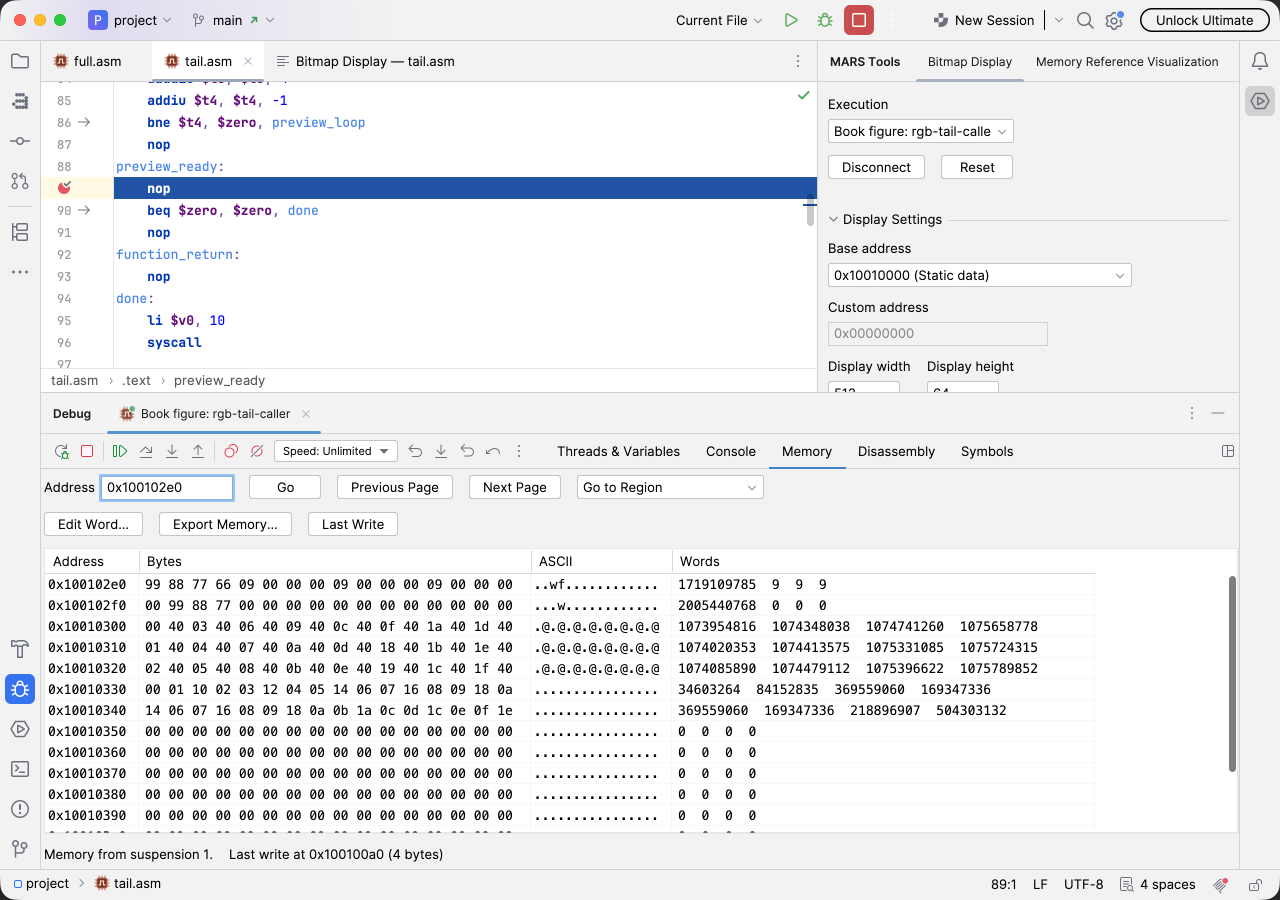
\includegraphics[artifact]{packages/019-rgb-formats/captures/f04/caller.png}}
\edef\MARSrgbtailsourceLeft{\the\dimexpr0.036718750\wd0\relax}
\edef\MARSrgbtailsourceBottom{\the\dimexpr0.774444444\ht0\relax}
\edef\MARSrgbtailsourceRight{\the\dimexpr0.713281250\wd0\relax}
\edef\MARSrgbtailsourceTop{\the\dimexpr0.170000000\ht0\relax}
\edef\MARSrgbtailregistersLeft{\the\dimexpr0.246093750\wd0\relax}
\edef\MARSrgbtailregistersBottom{\the\dimexpr0.334444444\ht0\relax}
\edef\MARSrgbtailregistersRight{\the\dimexpr0.553906250\wd0\relax}
\edef\MARSrgbtailregistersTop{\the\dimexpr0.640000000\ht0\relax}
\edef\MARSrgbtailbitmapLeft{\the\dimexpr0.032031250\wd2\relax}
\edef\MARSrgbtailbitmapBottom{\the\dimexpr0.405555556\ht2\relax}
\edef\MARSrgbtailbitmapRight{\the\dimexpr0.032031250\wd2\relax}
\edef\MARSrgbtailbitmapTop{\the\dimexpr0.428888889\ht2\relax}
\edef\MARSrgbtailpackedLeft{\the\dimexpr0.034375000\wd4\relax}
\edef\MARSrgbtailpackedBottom{\the\dimexpr0.311111111\ht4\relax}
\edef\MARSrgbtailpackedRight{\the\dimexpr0.584375000\wd4\relax}
\edef\MARSrgbtailpackedTop{\the\dimexpr0.608888889\ht4\relax}
\edef\MARSrgbtailexpandedLeft{\the\dimexpr0.034375000\wd6\relax}
\edef\MARSrgbtailexpandedBottom{\the\dimexpr0.311111111\ht6\relax}
\edef\MARSrgbtailexpandedRight{\the\dimexpr0.584375000\wd6\relax}
\edef\MARSrgbtailexpandedTop{\the\dimexpr0.608888889\ht6\relax}
\edef\MARSrgbtailcallerLeft{\the\dimexpr0.034375000\wd8\relax}
\edef\MARSrgbtailcallerBottom{\the\dimexpr0.334444444\ht8\relax}
\edef\MARSrgbtailcallerRight{\the\dimexpr0.584375000\wd8\relax}
\edef\MARSrgbtailcallerTop{\the\dimexpr0.608888889\ht8\relax}
\begin{tikzpicture}[alt={Six annotated panels show a fresh nine-pixel run at preview_ready. Return and both caller result counts are nine. Each bitmap row contains nine selected colors followed by 23 untouched zero cells. Ninth packed pixel at 0x10010228 is bytes 08 42; ninth expanded RGB at 0x100101a8 is 42 41 42, or 66,65,66. Bytes beyond the logical outputs remain zero.}]
\node[anchor=north west,inner sep=0,font=\small\bfseries] (source-title) at (6mm,0) {Next instruction at this boundary};
\node[anchor=north west,inner sep=0] (source) at ([yshift=-1mm]source-title.south west) {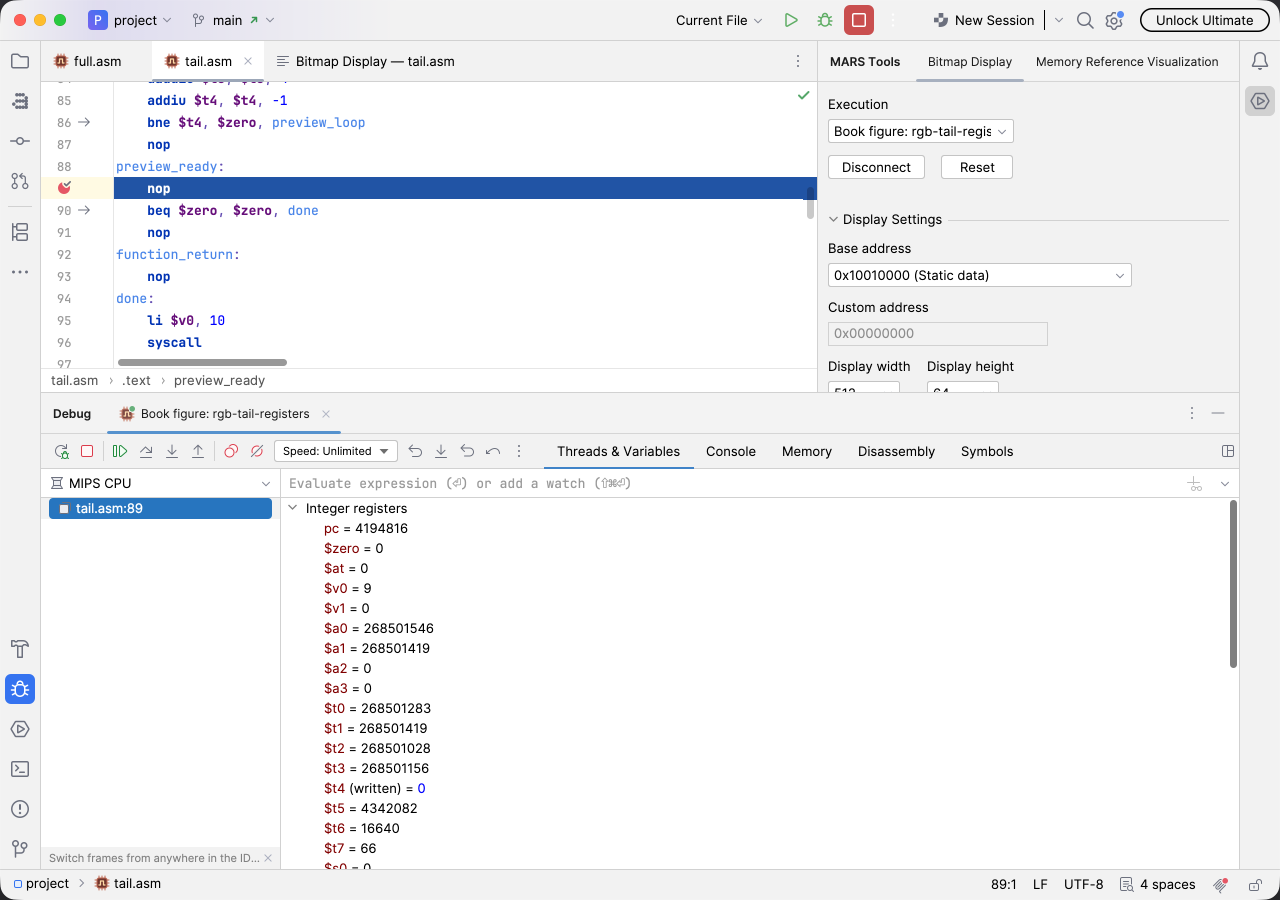
\includegraphics[width=0.54\linewidth,artifact,trim={\MARSrgbtailsourceLeft{} \MARSrgbtailsourceBottom{} \MARSrgbtailsourceRight{} \MARSrgbtailsourceTop{}},clip]{packages/019-rgb-formats/captures/f04/registers.png}};
\begin{scope}[shift={(source.south west)},x={($(source.south east)-(source.south west)$)},y={($(source.north west)-(source.south west)$)}]
\draw[black,line width=0.7pt] (0.215625000,0.080000000) rectangle (0.384375000,0.520000000);
\node[draw=black,fill=white,circle,inner sep=1.5pt,font=\footnotesize] at ($(0.215625000,0.520000000)+(-3mm,0)$) {1};
\end{scope}
\node[anchor=north west,inner sep=0,font=\small\bfseries] (registers-title) at (0.58\linewidth,0 |- source-title.north) {Returned pixel count};
\node[anchor=north west,inner sep=0] (registers) at ([yshift=-1mm]registers-title.south west) {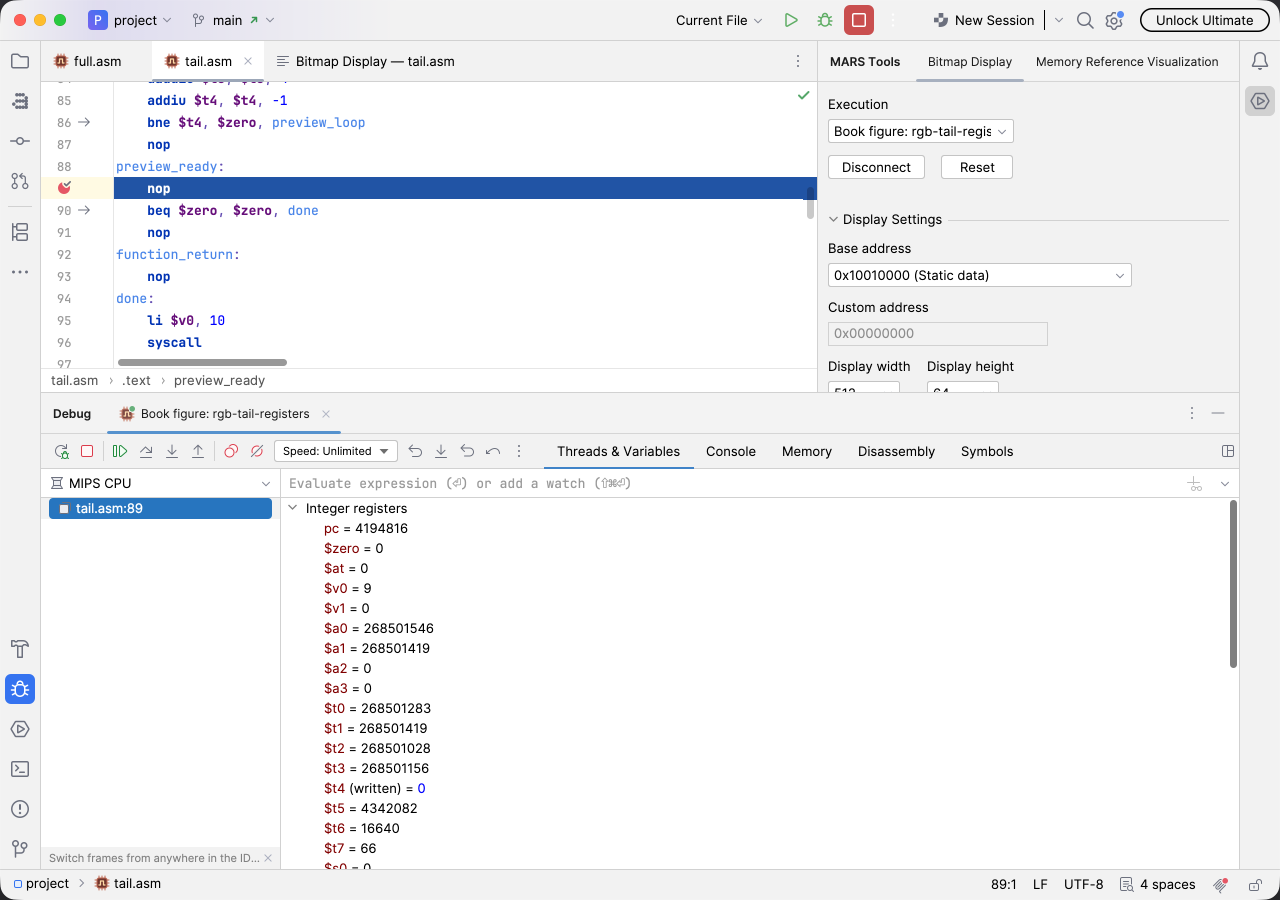
\includegraphics[width=0.42\linewidth,artifact,trim={\MARSrgbtailregistersLeft{} \MARSrgbtailregistersBottom{} \MARSrgbtailregistersRight{} \MARSrgbtailregistersTop{}},clip]{packages/019-rgb-formats/captures/f04/registers.png}};
\begin{scope}[shift={(registers.south west)},x={($(registers.south east)-(registers.south west)$)},y={($(registers.north west)-(registers.south west)$)}]
\draw[black,line width=0.7pt] (0.023437500,0.043478261) rectangle (0.226562500,0.913043478);
\node[draw=black,fill=white,circle,inner sep=1.5pt,font=\footnotesize] at ($(0.023437500,0.913043478)+(-3mm,0)$) {2};
\end{scope}
\node[anchor=north west,inner sep=0,font=\small\bfseries] (bitmap-title) at ([yshift=-1mm]source.south west) {Original row above the expanded row};
\node[anchor=north west,inner sep=0] (bitmap) at ([yshift=-1mm]bitmap-title.south west) {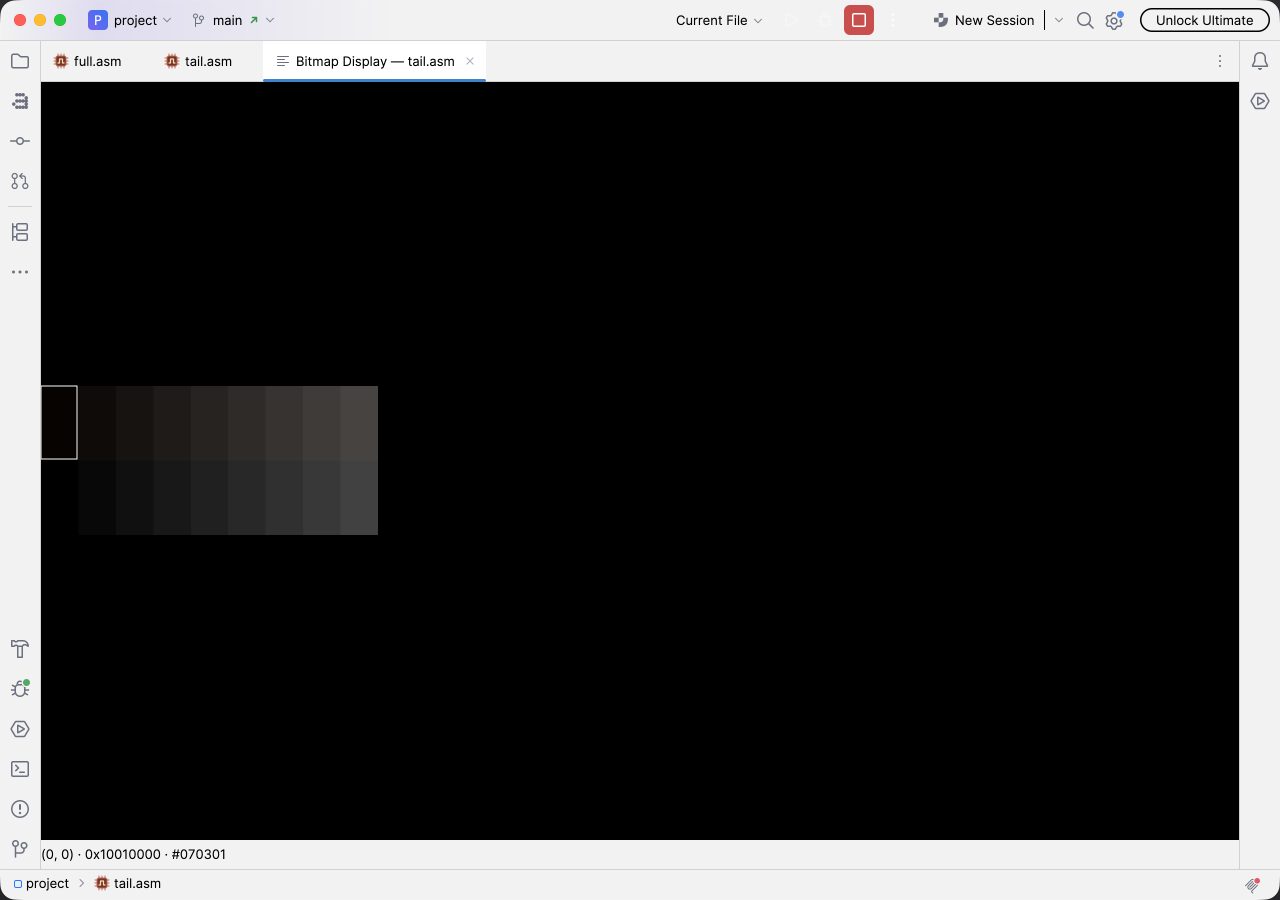
\includegraphics[width=0.84\linewidth,artifact,trim={\MARSrgbtailbitmapLeft{} \MARSrgbtailbitmapBottom{} \MARSrgbtailbitmapRight{} \MARSrgbtailbitmapTop{}},clip]{packages/019-rgb-formats/captures/f04/bitmap.png}};
\begin{scope}[shift={(bitmap.south west)},x={($(bitmap.south east)-(bitmap.south west)$)},y={($(bitmap.north west)-(bitmap.south west)$)}]
\draw[black,line width=0.7pt] (0.000000000,0.000000000) rectangle (1.000000000,1.000000000);
\node[draw=black,fill=white,circle,inner sep=1.5pt,font=\footnotesize] at ($(0,1.000000000)+(-3mm,0)$) {3};
\end{scope}
\node[anchor=north west,inner sep=0,font=\small\bfseries] (packed-title) at ([yshift=-1mm]bitmap.south west) {Low-byte-first RGB565};
\node[anchor=north west,inner sep=0] (packed) at ([yshift=-1mm]packed-title.south west) {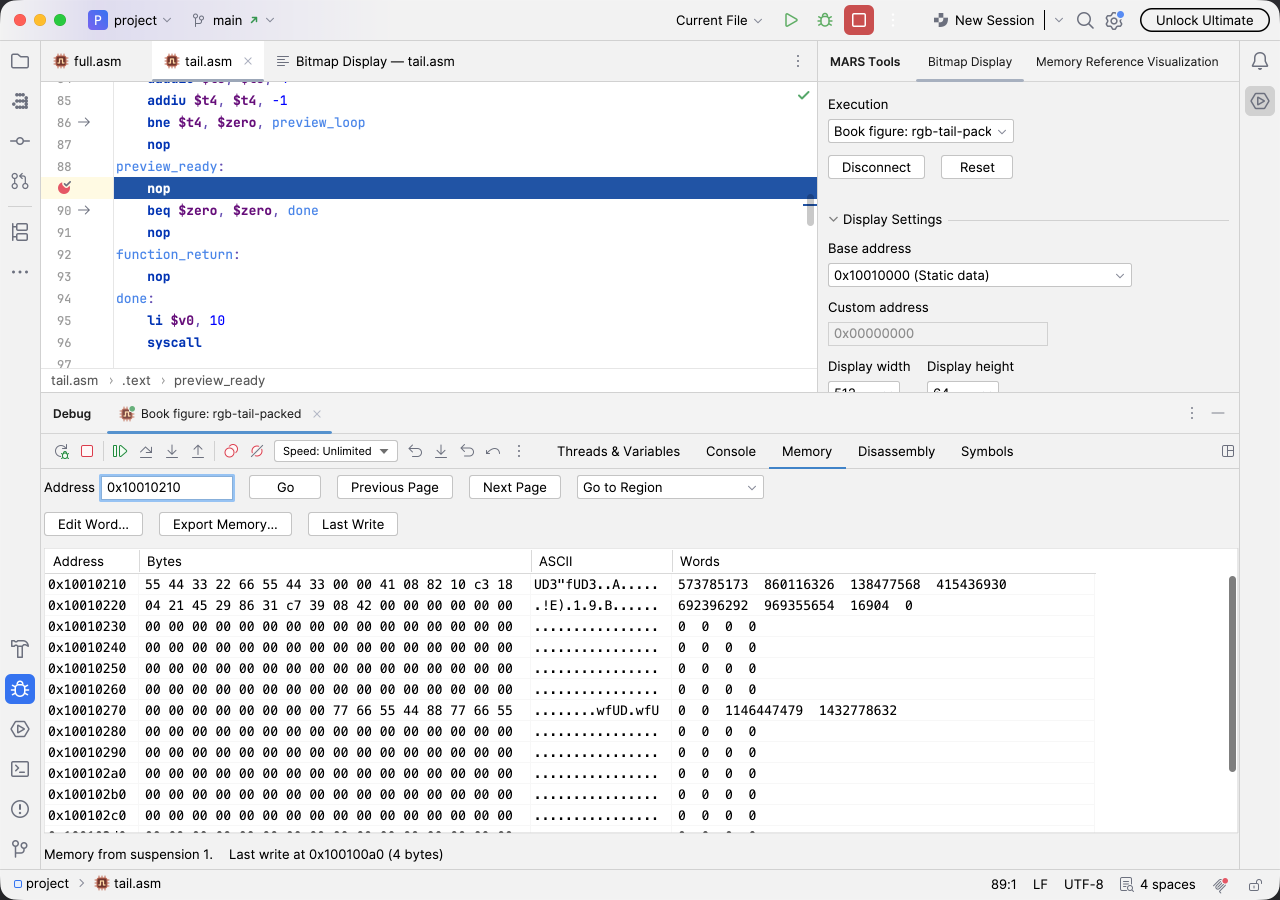
\includegraphics[width=0.84\linewidth,artifact,trim={\MARSrgbtailpackedLeft{} \MARSrgbtailpackedBottom{} \MARSrgbtailpackedRight{} \MARSrgbtailpackedTop{}},clip]{packages/019-rgb-formats/captures/f04/packed.png}};
\begin{scope}[shift={(packed.south west)},x={($(packed.south east)-(packed.south west)$)},y={($(packed.north west)-(packed.south west)$)}]
\draw[black,line width=0.7pt] (0.194672131,0.055555556) rectangle (0.997950820,0.638888889);
\node[draw=black,fill=white,circle,inner sep=1.5pt,font=\footnotesize] at ($(0,0.638888889)+(-3mm,0)$) {4};
\end{scope}
\node[anchor=north west,inner sep=0,font=\small\bfseries] (expanded-title) at ([yshift=-1mm]packed.south west) {Expanded RGB component bytes};
\node[anchor=north west,inner sep=0] (expanded) at ([yshift=-1mm]expanded-title.south west) {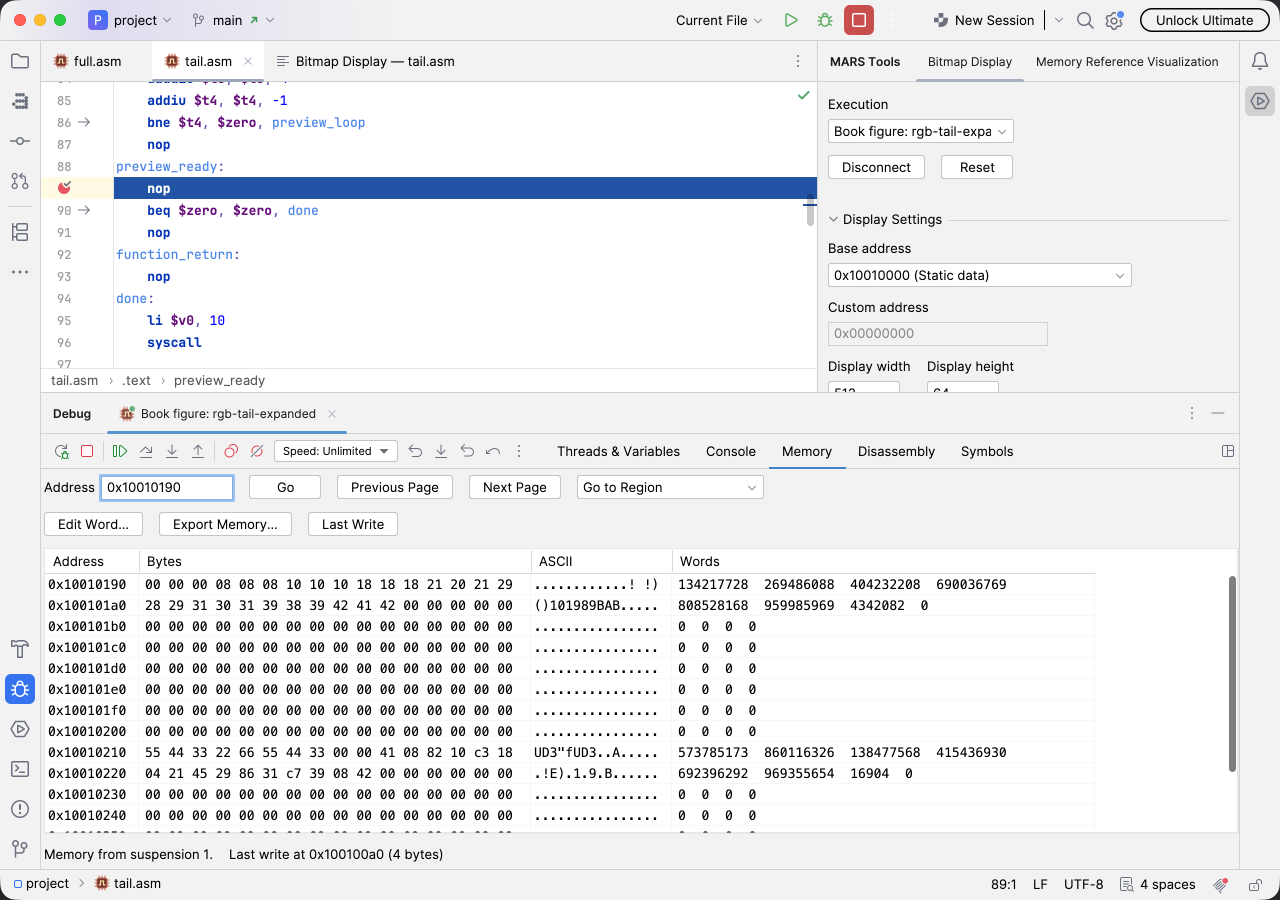
\includegraphics[width=0.84\linewidth,artifact,trim={\MARSrgbtailexpandedLeft{} \MARSrgbtailexpandedBottom{} \MARSrgbtailexpandedRight{} \MARSrgbtailexpandedTop{}},clip]{packages/019-rgb-formats/captures/f04/expanded.png}};
\begin{scope}[shift={(expanded.south west)},x={($(expanded.south east)-(expanded.south west)$)},y={($(expanded.north west)-(expanded.south west)$)}]
\draw[black,line width=0.7pt] (0.194672131,0.055555556) rectangle (0.997950820,0.638888889);
\node[draw=black,fill=white,circle,inner sep=1.5pt,font=\footnotesize] at ($(0,0.638888889)+(-3mm,0)$) {5};
\end{scope}
\node[anchor=north west,inner sep=0,font=\small\bfseries] (caller-title) at ([yshift=-1mm]expanded.south west) {Count and caller result words};
\node[anchor=north west,inner sep=0] (caller) at ([yshift=-1mm]caller-title.south west) {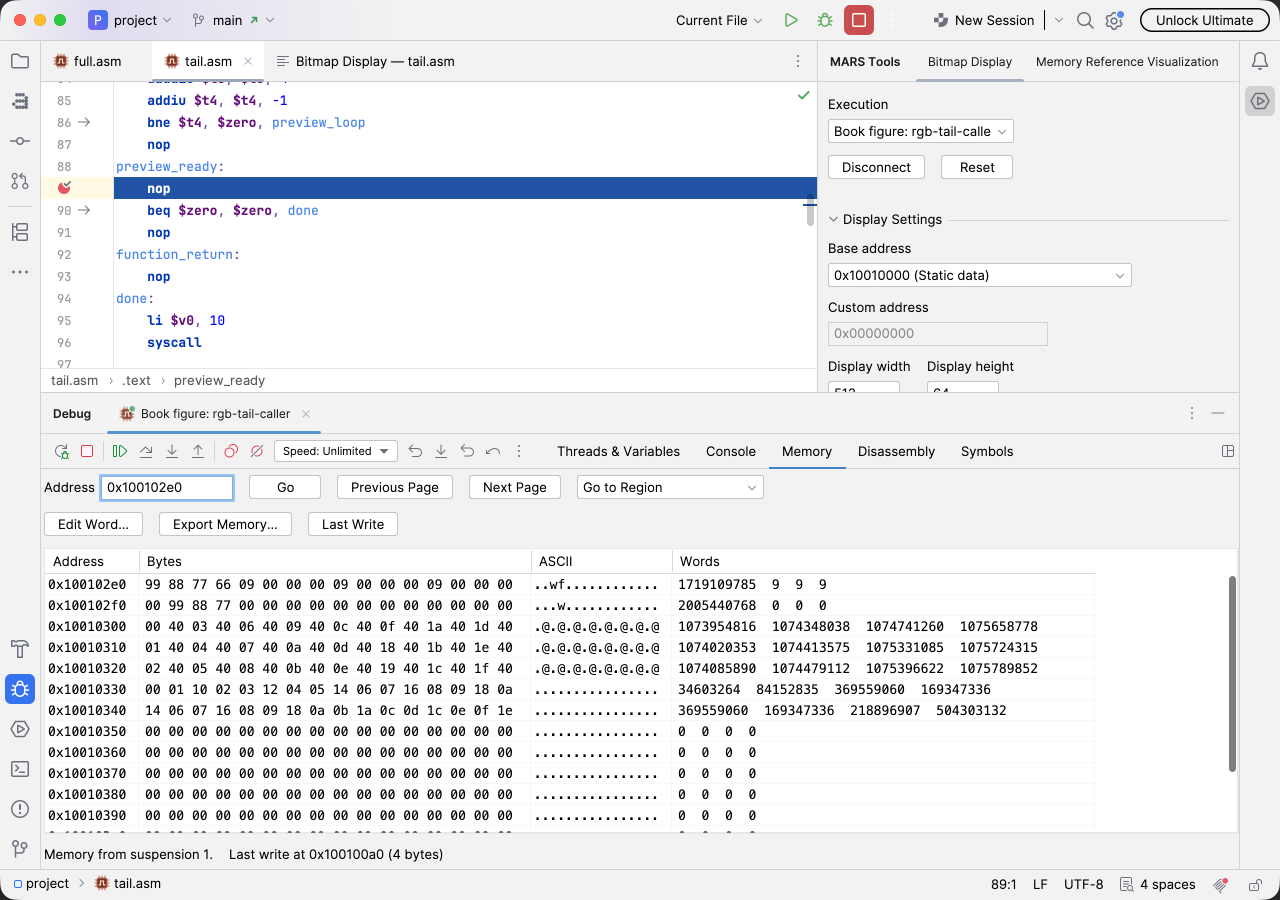
\includegraphics[width=0.84\linewidth,artifact,trim={\MARSrgbtailcallerLeft{} \MARSrgbtailcallerBottom{} \MARSrgbtailcallerRight{} \MARSrgbtailcallerTop{}},clip]{packages/019-rgb-formats/captures/f04/caller.png}};
\begin{scope}[shift={(caller.south west)},x={($(caller.south east)-(caller.south west)$)},y={($(caller.north west)-(caller.south west)$)}]
\draw[black,line width=0.7pt] (0.194672131,0.078431373) rectangle (0.997950820,0.490196078);
\node[draw=black,fill=white,circle,inner sep=1.5pt,font=\footnotesize] at ($(0,0.490196078)+(-3mm,0)$) {6};
\end{scope}
\end{tikzpicture}
\par\smallskip
\begin{minipage}{\linewidth}
\small
\begin{enumerate}
\setlength{\itemsep}{2pt}
\setlength{\parsep}{0pt}
\item This fresh run changes only count to 9. The guided conversions handle one eight-pixel vector group and one scalar tail pixel. The same \texttt{preview\_ready} marker follows both conversions and the caller\textquotesingle s display loop.
\item \texttt{\$v0 = 9} counts pixels. Packing reads 27 bytes and writes 18; expansion reads 18 and writes 27. A mapped allocation is larger than these logical slices, so nearby accessible bytes do not authorize a wider tail access.
\item Each row contains nine selected pixels followed by 23 untouched zero cells. The first expanded pixel is also black, so black appearance alone cannot identify padding. The returned count and bounded access history establish the nine-pixel extent.
\item The ninth packed pixel is at \texttt{0x10010228}, sixteen bytes after the output base. Bytes \texttt{08 42} encode \texttt{0x4208}. Following zeros are outside the eighteen-byte output and remain unchanged; they are not additional converted pixels.
\item The ninth expanded triple at \texttt{0x100101a8} is \texttt{42 41 42}, or $(66,65,66)$. Its original $(71,67,65)$ cannot be recovered after quantization. These three scalar-tail stores finish the 27-byte output without touching its suffix.
\item The caller row contains count 9, packed result 9 and expanded result 9 after its guard. Complete images and access traces also check unseen suffixes, other buffers, guards and constant masks, including stores that would leave the same byte value.
\end{enumerate}
\end{minipage}
\caption{Nine pixels exercise one vector group and one scalar tail without extending the slices.}
\label{capture:019-rgb-formats-f04}
\label{rgb-f04}
\end{figure}
\par
